\clearpage
\chapter{\textbf{Implementation}}\label{Implementation}
\subsubsection{Sewing Machine Signal Connection and Data Acquisition}
The final signals necessary to calculate all selected KPIs are "Thread Trimming," "Pressure foot," "Upper shaft rotating," and "Main menu and not sewing." The retrieval of these signals was contingent upon their initial assignment to the correct output pins in the machine's menu configuration. The subsequent challenge was to establish a connection between the output pins and the input pins of the WAGO PLC.

A connection for one signal from the sewing machine had already been established during an earlier project, but unfortunately, the connection was inadequately documented. This proved to be more confusing than helpful. The connection was implemented as follows: The signal pin of the sewing machine was connected to the 0V reference of the PLC. The 24V pin of the sewing machine was connected to the signal input connector of the PLC. Figure 5.1 provides a visual aid to facilitate comprehension of this configuration. This arrangement made sense once it was discovered that the sewing machine signals are NPN type, while the PLC exclusively accepts PNP signals as input. Typically, when the sewing machine would also have signals of type PNP, the signal pins would simply be connected to the signal connectors of the PLC. Concurrently, the 0V connector of the PLC would be connected to the GND pin of the sewing machine.
\begin{figure}[H]
	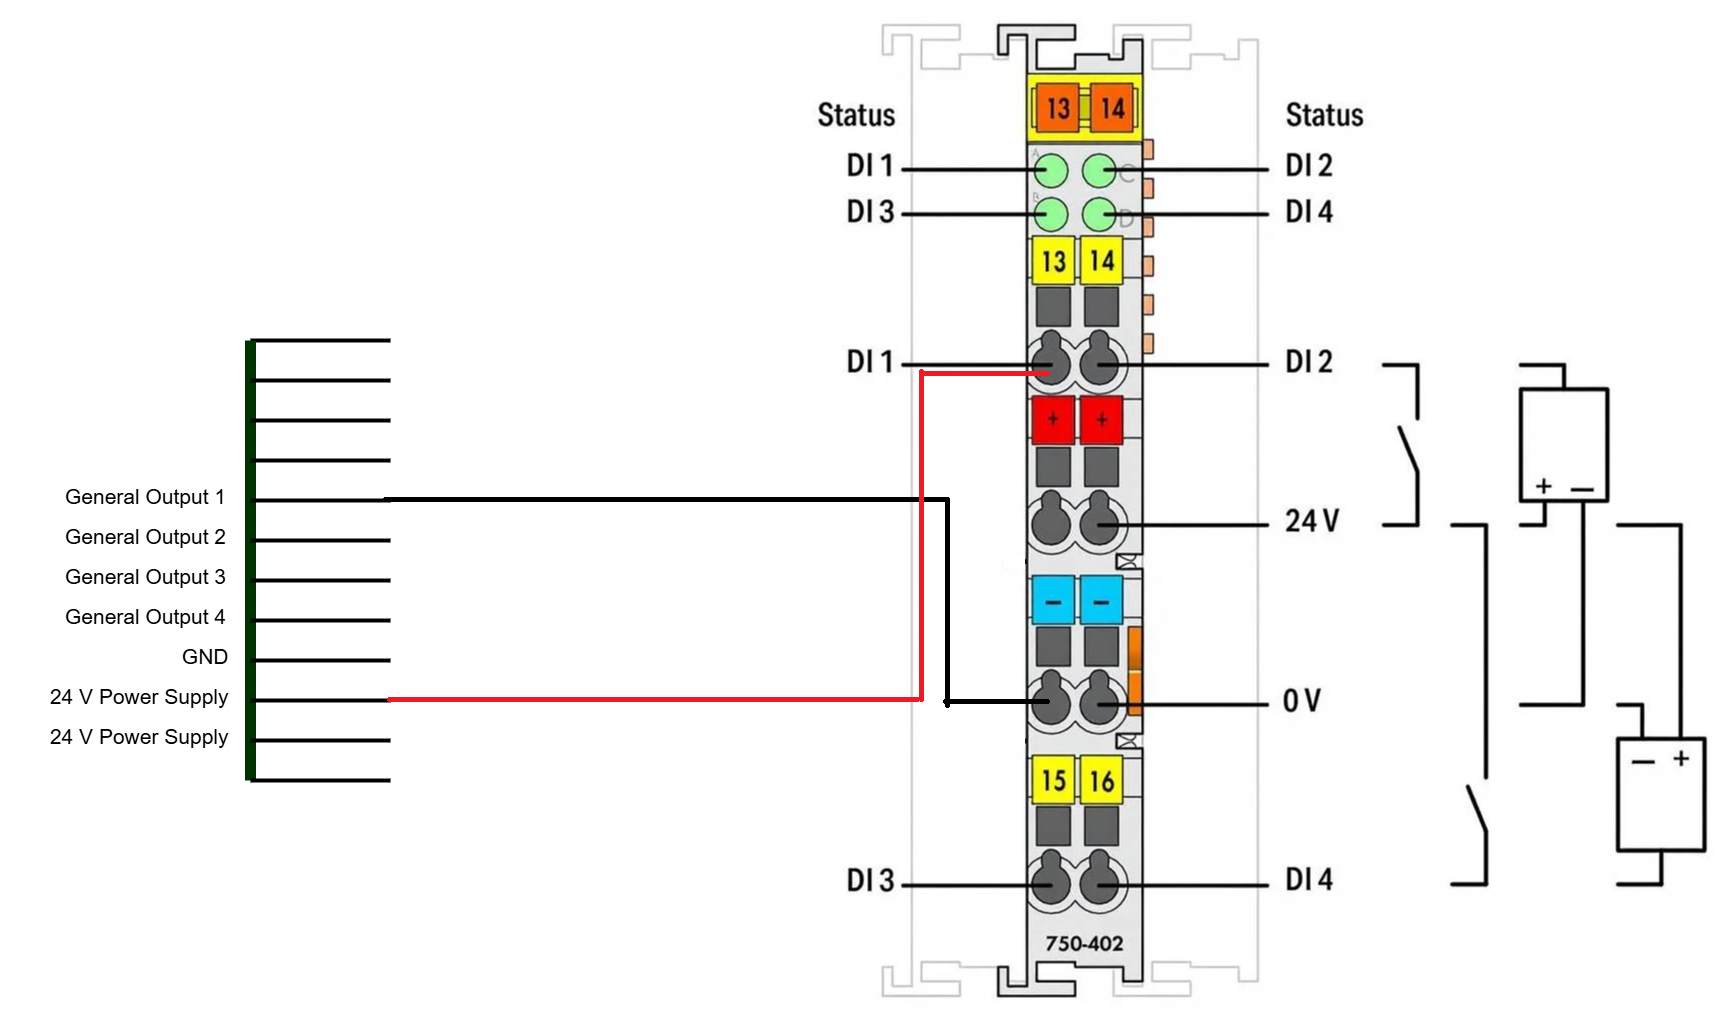
\includegraphics[height=7.4cm]{pic/sewing-machine-plc-init.png}
	\caption{Initial Connection of Sewing Machine to PLC}
	\label{fig:Model-Component-Pattern}
	\small\textit{Note: The 12-pin connector of the sewing machine is located on the left side. This connector contains various pins, including those that function as signal pins. The left side of the module contains the PLC input module. The DI1-4 marked connectors of the PLC serve the function of signal input connectors.}
\end{figure}
The system was configured so that when a signal becomes active, it draws current through the signal input connector of the PLC, resulting in a high signal. However, this implementation was limited to only two signals, because there is only one 0V connector available for two signal input connectors. In total, there are two 0V connectors and four signal input connectors. When two 24V pins are connected to one 0V connector via the signal input pins, an active signal draws current through the 0V connection and simultaneously pulls current from both input signal connectors. This results in invalid signals. 


The resolution of the aforementioned issue necessitated the conversion of the NPN signals of the sewing machine into PNP signals, which are compatible with the PLC. For the execution of this task, an optocoupler was utilized. The implementation was executed in accordance with the subsequent description. Subsequently, the signal output pins of the sewing machine were connected to the signal input connectors of the optocoupler. Furthermore, a connection to the 24-V power supply of the sewing machine was established for each signal input. The signal connectors on the output side of the optocoupler are connected to the signal input connectors of the PLC. Concurrently, the 24-V power supply of the PLC is connected to the VCC input connector of the optocoupler. Additionally, the 0V connector of the programmable logic controller PLC is linked to the GND connector of the optocoupler. The wiring of the optocoupler can be observed in the following Figure.
\begin{figure}[H]
	\centering
	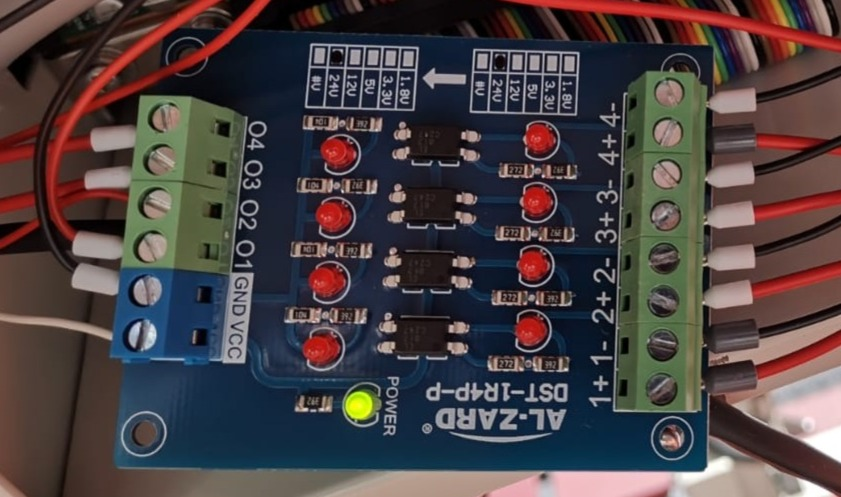
\includegraphics[height=6cm]{pic/optocoupler-wiring.jpg}
	\caption{Initial Connection of Sewing Machine to PLC}
	\label{fig:Model-Component-Pattern}
\end{figure}
As illustrated, the red cables represent electrical connections originating from or terminating at a 24V power source. Additionally, the white cable located on the left side is linked to the 24V source of the PLC. The black cables serve as connections to ground or to the signal pins on the right side. These connections function in a manner that pulls down the current when signals are in a state of activity.
In order to ensure the signal's availability across the shopfloor network, it was imperative to program the PLC in a manner that facilitated this objective. The input signals simply needed to be assigned to a value and then published over OPC UA. \\
Initially, only the IP address and the OPC UA port of the PLC were known. In order to enhance comprehension regarding the retrieval of data from the aforementioned system through the utilization of an OPC UA client, the development of a Python script was undertaken. The script under consideration took the two givens, established a connection, and navigated through the OPC UA server's node structure. The search is conducted for a "DeviceSet" node, which is understood to generally contain industrial devices, such as sewing machines. For each device identified, an exploration of its variables and child objects is initiated. It is important to acknowledge that, at this juncture, the connection from the preceding project was still in place. Further exploration was necessary to ascertain the nature of the connection and to identify any additional machines that were connected to the PLC. At this time there was a delay in communication with "Brother Internationale Industriemaschinen GmbH." Therefore, the necessary information regarding the configuration of the sewing machine signals was not available. A decision was reached to initiate an exploration of effective communication methods with the OPC UA server.\\
Subsequent to the establishment of a connection to the PLC for all signals, a diagnostic procedure was conducted to ascertain the availability of all signals. For this purpose, a tool known as UAExpert was utilized. The software under discussion is an OPC UA client that provides a user interface for development, testing, and monitoring. The device was utilized for the purpose of monitoring the values of the signals. Consequently, the actions that were expected to elicit the signals were executed on the sewing machine. Initially, the process was proceeding according to plan. -	However, after a certain period, one of the signals ceased functioning, resulting in a persistent display of the value "false". Therefore, it was necessary to measure the current in order to ascertain the location of the failure. It was observed that a short circuit occurred on the printed circuit board (PCB) during the measurement process. The probable rationale pertains to an inadvertent connection between two 24-volt sources through the utilization of a multimeter.  Subsequent to the incident, retrieval of the signals from the sewing machine was rendered unfeasible. A decision was made to simulate the OPC UA server and generate test data that would emulate the standard sewing process. The decision was made to implement the system in a manner that would allow for the subsequent connection of the sewing machine to the data processing and analytics system following the installation of a new PCB.

\subsection{Data preprocessing}
\begin{figure}[H]
	\centering
	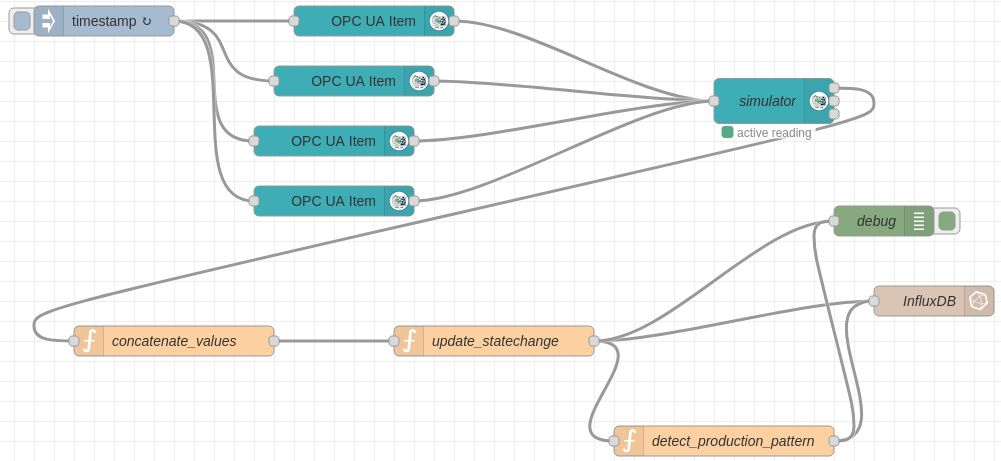
\includegraphics[height=7cm]{pic/node-RED.jpg}
	\caption{Data retrieval and preprocessing}
	\label{fig:Model-Component-Pattern}
\end{figure}
In the context of this study, Node-RED was utilized as a service to retrieve data that had been published by the PLC's OPC UA server. This feature facilitates the preprocessing and subsequent injection of data into the database. The retrieval of data from the OPC UA server is facilitated by an OPC UA package known as "node-red-contrib-opcua." The node designated as "timestamp" at the inception of the flow serves merely to initiate the flow. The temporal configuration of this feature may be set to various intervals or fixed times. The decision was made to establish an interval of 0.2 seconds. This interval was selected due to the fact that some operations on the sewing machine have an execution time of approximately one second when operated by inexperienced workers. In light of the dearth of seasoned professionals, it was deduced that an experienced worker would exhibit a fourfold increase in efficiency. To ensure the capture of all events, the interval was set to 0.2 seconds, equivalent to the execution time of a worker operating at a rate five times faster. Subsequent to the completion of the trial, the interval may be recalibrated in accordance with the findings of the evaluation. The four subsequent nodes, designated as OPC UA Items, each contain the namespace and ID of the various signals. These are subsequently fed into the simulator node. The node in question has been configured with the endpoint, which consists of the IP address of the PLC, the port, and the name of the OPC UA server, if such a server exists. This node is responsible for generating the values for each of the OPC UA items in a serial manner.
The succeeding node is one of three function nodes. These function nodes contain JavaScript code that executes three distinct preprocessing steps. The initial step involves the concatenation of the four values into a single string. The primary rationale for concatenating values is that, in InfluxDB, each value is assigned its own table. In the event that a query is executed over a set of values, the tables must be joined, a process that is computationally intensive. This phenomenon can result in substantial delays in the final dashboard. The concatenation of values eliminates the necessity for joining tables, as all values are subsequently stored within a single table.
This preprocessing step confers an additional advantage, namely that it facilitates the subsequent step in the procedure. The subsequent preprocessing step in the function node designated "update\_statechange" involves the verification of whether the concatenated string undergoes alterations. A modification in the configuration of the string is indicative of a state alteration in the sewing machine. Consequently, the string undergoes an output transformation. The initial concatenation of the values reduces the number of comparisons from four to one string. This preprocessing step was implemented to reduce the amount of data stored in the database. In previous iterations, this step was omitted, resulting in a substantial reduction in query processing speed relative to subsequent iterations. The output of the second preprocessing node is comprised of four separate key-value pairs of the signals, as well as these in a concatenated string format. It is important to note that these values are only provided as output when there is a change in one of the values compared to the previous state. The output of this node is utilized as an input for the third preprocessing node.
In the preceding section (4.0.7), the production pattern was delineated as a metric for quantifying the duration of machine utilization for value-adding operations. The final preprocessing node, designated "detect\_production\_pattern", serves to ascertain the presence of this pattern. The output of this function is the key "pattern" with a value of true, indicating the beginning of the pattern, or false, indicating the end of the pattern. Additionally, the timestamp indicating the end or beginning of the pattern is included in the output.
Upon completion of the data flow, both outputs from the "updateStateChange" function and the "detect\_production\_pattern" process are transferred to the designated InfluxDB node as input. This node has been configured with the address and the API key of the Influx database. The component in question is an InfluxDB out node, which signifies that it is capable of writing data exclusively to InfluxDB. This node stems from the node-red-contrib-influxdb package. In the course of each write operation, the system automatically incorporates a timestamp into the input. However, it is imperative to incorporate a timestamp at the "detect\_production\_pattern" node, as the pattern's detection is only possible in a retrospective manner. Consequently, the timestamp of the InfluxDB node would be inadequate.




